%!TEX root = ../Main.tex

%-------------------------------------------------------------------------------

\chapter{Clustering Methods}
Clustering refers to grouping data into different clusters or classes. We do this to get observations or samples clustered into groups where they share some similarities. This is used extensively in the field of machine learning. An example of clusters or classes could be handwritten numbers (0-9). Each number has distinct features which can be divided into clusters. An unsupervised problem would be to divide the numbers into subclasses. In a supervised problem we would already have made the clustering and then divide new samples into the already known clusters, or in other words, predict some outcome based on the sample.

\section{K-means clustering}
K-means clustering is a simple method of clustering data. It works by having a number (K) mean-vectors and assigning a sample to the mean-vector that it's closest to. On \cref{fig:k-means_clustering} 150 sample have been generated and three different values for K. It is easy to see that the K-means method tries to cluster samples that are close to each other in the same class.

\begin{figure}[H]
	\centering
	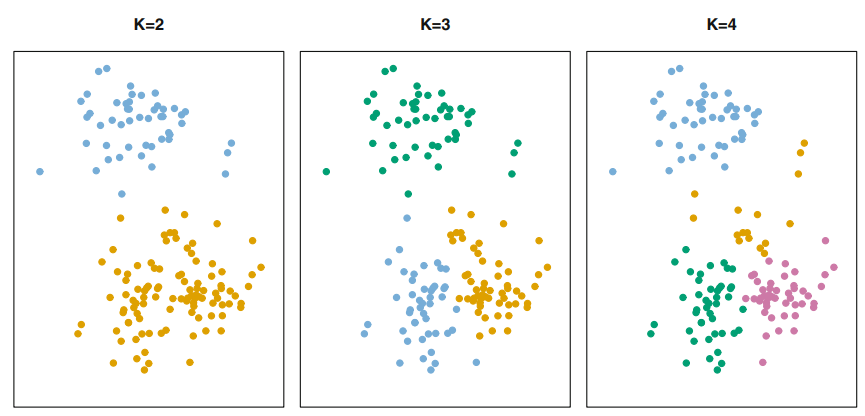
\includegraphics[width=12cm]{Img/K-means_clustering.PNG}
	\caption{K-means clustering example}
	\label{fig:k-means_clustering}
\end{figure} 

This works by minimizing the squared euclidean distance to each mean-vector. 

\begin{equation} \label{transformed_linear_regression_eq}
minimize_{C1...C_{K}}\{\sum_{k=1}^{K}\dfrac{1}{\lvert C_{k} \rvert} \sum_{i,i'\in C_{k}}^{} \sum_{j=1}^{p}(x_{ij}-x_{i'j})^{2} \}
\end{equation}

$\lvert C_{k}\rvert$ denotes the number of samples in the kth cluster. Or the within variation of the kth cluster which is the sum of all the pairwise squared euclidean distances between the samples in the kth cluster, divided by the total number of samples in kth cluster.

To implement this as an algorithm the book \cite{book_2015} covers how this should be done. 

\begin{figure}[H]
	\centering
	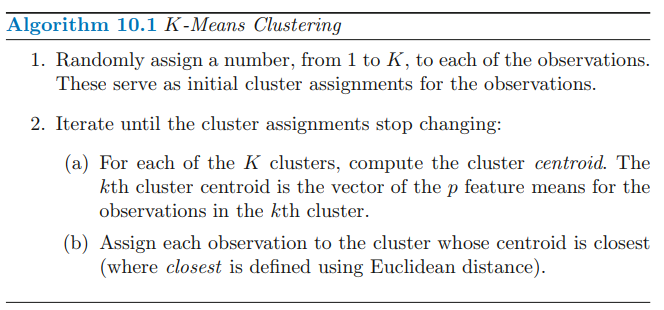
\includegraphics[width=12cm]{Img/Algo_kmeans.PNG}
	\caption{K-means clustering pseudo code}
	\label{fig:k-Algo_kmeans}
\end{figure} 

In action this algorithm performs well and can be seen on \cref{Algo_kmeans_inaction}

\begin{figure}[H]
	\centering
	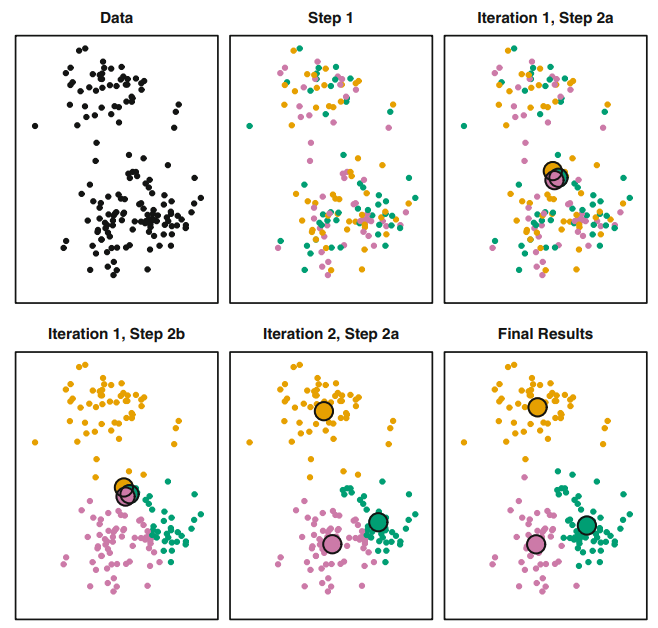
\includegraphics[width=10cm]{Img/Kmean_algo_example.PNG}
	\caption{K-means clustering in action}
	\label{fig:k-Algo_kmeans_inaction.PNG}
\end{figure} 


\subsection{Hierarchical Clustering}
Hierarchical Clustering makes use of tree-based representation of the samples. This tree-based representation is called a Dendrogram and looks like an upside-down tree. An example of a dendrogram can be seen on \cref{fig:dendrogram}\cite{book_2015}


\begin{figure}[H]
	\centering
	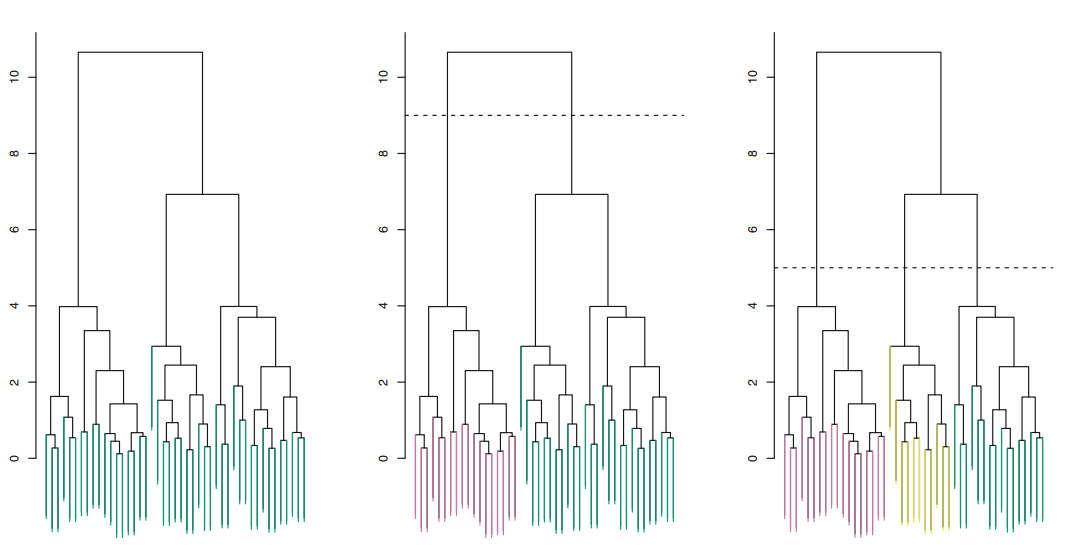
\includegraphics[width=10cm]{Img/Dendrogram_example.PNG}
	\caption{Dendrogram example}
	\label{fig:dendrogram}
\end{figure} 

Its easy to see how the clustering works. It starts from the bottom works its way up. To see if two samples are similar we can compare how far up on the vertical axis two samples fuses. If they fuse at the bottom they are very similar and at to top not very similar. 

A hierarchical clustering algorithm will work like the dendrogram. That means that if we have \textit{n} sample, it will also starts at the bottom and look at the two samples that are most similar and fuses them together so we have n-1 clusters. Next it will again fuse the two most similar samples and will be left with n-2 clusters. The algorithm will keep going until all samples belong to a cluster. 
 


\section{Lab results}

The data for the two lab exercises 10.5.1 and 10.5.2 are generated with the code listed in \ref{lst:data_gen}. The data is made so that it contains two natural clusters.\\ 
Performing KMeans on the generated data with k = 2 and k = 3 both with 20 random initial assignments results in the data clustering on figure \ref{fig:KMeans}. For k = 2 the data is clearly divided into two clusters (red and green), while for k = 3 it is divided into three clusters (red, green and yellow). Adding additional clusters also results in different cluster means as is evident by the black +, which denotes the given clusters mean.\\
Figure \ref{fig:HC_Complete} shows the "complete"\ hierarchical clustering of the data, which is generated as "bottom up"\ clustering by comparing the largest pairwise distance between points in possible clusters. The colors red and green marks the two clusters that is known to be in the data, while the blue color marks the "single cluster" being all the data.\\ 
Using "single"\ hierarchical clustering of the data, the graph would instead show clustering by comparing the smallest pairwise distance between points in possible clusters. Lastly also "average"\ hierarchical clustering could be used, which of course would use the average distance instead.


\begin{lstlisting}[language=Python, caption=Code for generating the data]
# Generate data
np.random.seed(2)
X = np.random.standard_normal((50,2))
X[:25,0] = X[:25,0]+3
X[:25,1] = X[:25,1]-4
\end{lstlisting}\label{lst:data_gen}


\begin{figure}[H]
	\centering
	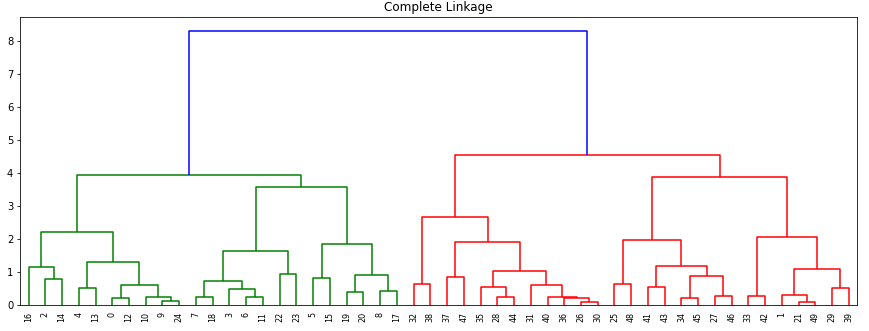
\includegraphics[width=14cm]{Img/HC_Complete.PNG}
	\caption{Complete histogram of clusters in the data set}
	\label{fig:HC_Complete}
\end{figure}

\begin{figure}[H]
	\centering
	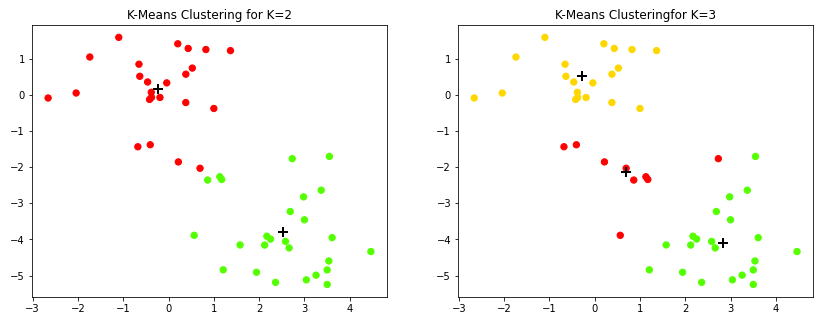
\includegraphics[width=14cm]{Img/KMeans.PNG}
	\caption{Clusters generated by KMeans with k = 2 and k = 3}
	\label{fig:KMeans}
\end{figure} 

